%%%%%%%%%%%%%%%%%%%%%%%%%%%%%%%%%%%%%%%%%%%%%%%%%
% MANUSCRIPT TEMPLATE: This is the official manuscript template (v1.0, released 31 August 2025) for Constitutional Studies. If you are new to using LaTeX to layout manuscripts in Overleaf, please read this helpful tutorial at www.overleaf.com/learn/latex/Learn_LaTeX_in_30_minutes. For more on Constitutional Studies, visit constitutionalstudies.org.

% TO PREPARE YOUR MANUSCRIPT: Review our manuscript guidelines at https://constitutionalstudies-ojs-utexas.tdl.org/cs/manuscriptguidelines. Then follow the instructions in green below at the beginning of each section.

% TO SUBMIT YOUR MANUSCRIPT: Follow our submission process at https://constitutionalstudies-ojs-utexas.tdl.org/cs/submit.
%%%%%%%%%%%%%%%%%%%%%%%%%%%%%%%%%%%%%%%%%%%%%%%%%

% DOCUMENT SETUP: Do not make any changes to this section.
\documentclass[a4paper,10.5pt,twoside]{article}
\hyphenpenalty=8000
\textwidth=125mm
\textheight=200mm
\usepackage[top=3cm, bottom=3cm, inner=3cm, outer=3cm, includehead]{geometry}
\usepackage{fancyhdr}
\pagestyle{fancy}
\fancyhead{}
\fancyfoot{}
\raggedbottom
\usepackage{xurl}
\usepackage{graphicx}
\usepackage{subcaption}
\usepackage{alltt}
\usepackage{booktabs}
\usepackage{float} 
\usepackage{amsmath}
\usepackage[hidelinks, pdftex]{hyperref}
\usepackage{amsfonts}
\urlstyle{same}
\usepackage[T1]{fontenc}
\usepackage[utf8]{inputenc}
\usepackage{lmodern}
\usepackage{csquotes}
\usepackage[notes, backend=biber]{biblatex-chicago}
\addbibresource{references.bib}
\pagenumbering{arabic}
\setcounter{page}{1}


% LANGUAGE SELECTION: If you are submitting your manuscript in English, do not make any changes to this section. If you are submitting your manuscript in French, add a % in front of the "\usepackage[english]{babel}" command and remove the % in front of the "\usepackage[french]{babel}" command below; this will apply French spelling and formatting rules to the document. If you are submitting your manuscript in Spanish, add a % in front of the "\usepackage[english]{babel}" command and remove the % in front of the "\usepackage[spanish]{babel}" command below; this will apply Spanish spelling and formatting rules to the document.
\usepackage[english]{babel}
%\usepackage[french]{babel}
%\usepackage[spanish]{babel}

% AUTHOR AND TITLE: Replace "Author1" with your first author's information where noted below. Add or remove additional author information as needed, depending on the number of authors on your manuscript. Replace "Article title" with your article title where noted below.
\begin{document}
\fancyhead[LE]{\thepage\ \ \ \   }
\fancyhead[RO]{Numerical Analysis, COS 574, (2025)\ \ \ \ \thepage}
\begin{center}
\LARGE
\textbf{ In-Game Chat Toxicity Intent Classification} \\[12pt]
\normalsize
\textbf {Cameron Letendre}\\[4pt]
\end{center}

% ABSTRACT AND KEYWORDS: Replace "Abstract text" with your abstract text of 100-200 words where noted below. Replace "keyword, keyword, keyword" with your 5-10 keywords, separated by commas, where noted below. 
\begin{abstract}
\normalsize
Inside this paper we explore the possibility of creating a more accurate prediction of toxicity in gaming messages, while trying to preserve speed for a real-time overlay. Modern gaming is known to be very structurally different from common language, but more than that because of the heavy involvement of slang, acronyms, and in-game vocabulary along with an average of 4 characters per message this creates a challenge for machine learning to predict the meaning of utterances. In this paper we attempt to do intent classification for predicting them into one of four groups: (E) Explicit Toxicity, (I) Implicit Toxicity, (A) Action, and (O) Other. This classification task for this assignment is done by a DistilBERT model that is fine-tuned on a labeled dataset known as CONDA. We additionally test whether normalised game-time context, prepended to each message as [TIME=x.xx], can help for the loss of conversational context that occurs when classifying messages one at a time, and report a small but consistent negative result.
\vspace{1em}
\end{abstract}

% MAIN BODY: Replace "Section Title," "Subsection Title," and "Subsubsection Title" with your section, subsection, and subsubsection titles, using title case to capitalize the first and all major words in these titles. Replace lorem ipsum text with your text for each section and subsection. Add additional sections and subsections as needed.
\section*{Introduction}

In competitive online games one of the greatest problems that exists is the involvement of harassment, slurs, and bullying in chat messages that riddles communications in online games. This is a well documented issue that has measurable effects on player retention and mental wellbeing. The Anti-Defamation League's 2020 \emph{Free to Play?} report found that 81\% of U.S.\ adult online multiplayer gamers had experienced some form of in-game harassment and 68\% had experienced severe forms (physical threats, stalking, or sustained harassment); among the fifteen titles surveyed, Dota 2 and VALORANT had the highest per-game harassment rates at 80\% each \autocite{adl2020freetoplay}.
\vspace{1em}

Existing mitigations are typically either proprietary client-side keyword filters, which are brittle and easily circumvented, or offline analyses on logs, which provide post-hoc insight but cannot intervene during play. 
\vspace{1em}

The goal I am trying to reach is an end-to-end system that can observe a live game, identify chat utterances on screen, and attempt to classify in near real-time. This helps with one of the bigger issues in this area which is the use of implicit toxicity which is less direct and harder to identify. For this system it requires combining computer-vision capture and low-latency NLP. These present the common questions of how we should handle OCR noise, how to keep the loop fast enough to be useful, and how can additional non-textual signals available from the game (timing, score, match state) improve classification beyond what text alone provides?
This project answers those questions in the context of CONDA (Weld et al., 2021), a publicly released dataset of 44,869 dual-annotated Dota 2 utterances. What we are trying to contribute is:

\begin{itemize}
    \item \textbf{A live capture-to-overlay pipeline.} Implements, end-to-end OCR to overlay:
        \begin{center}
            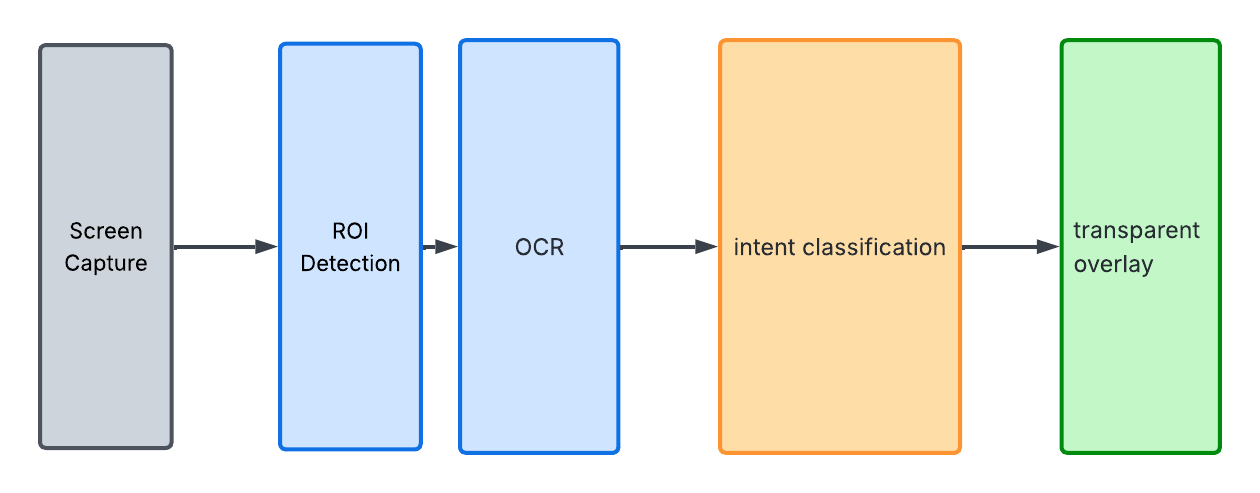
\includegraphics[width=0.80\linewidth]{end-to-end.png}
        \end{center}
        a transparent overlay engineered to skip redundant work from frame differencing and prediction caching.
    \item \textbf{A competitive single-task DistilBERT baseline on CONDA.} Trained on intent labels only, our model reaches macro-F1 0.8375 / UCA 0.9133 on the validation set, within 0.8 UCA points of CONDA's dual-task JointBERT baseline despite the absence of slot-level supervision.
    \item \textbf{A game-time conditioning ablation.} Tested whether a normalised match-time token, added as \texttt{[TIME=x.xx]} at the start of each utterance, can help for the loss of conversational context that occurs in real-time deployment. In this research we find that it does not: every per-class F1 drops.
    \item \textbf{An honest characterisation of the system's limitations,} including untested cross-game transfer (Dota training, VALORANT deployment) and pixel-coordinate-bound ROI.
\end{itemize}


\section{Related Work}

\textbf{The CONDA dataset} Weld et al. (2021) introduced CONDA, a dataset of in-game chat logs annotated for utterance-level intent (E / I / A / O) and token-level tags. Their published baselines include a:
Vanilla BERT classifier 
JointBERT model that performs intent and slot tagging in a single multi-task setup
The JointBERT model, which we treat as our reference baseline, reports UCA 0.921 with per-class U-F1 of 0.872 (E), 0.768 (I), 0.800 (A), and 0.954 (O) on the held-out test set.
\vspace{1em}

\textbf{Temporal patterns in toxicity}. Märtens et al. (2015) examined toxicity in Dota 2 matches and showed that toxic messages cluster around in-game events, such as post-death and post-team-fight moments, rather than uniformly across a match timeline. This was what motivated the hypothesis that match time, when supplied to an utterance, might provide a useful context about what utterances are likely to be toxic.
Distilbert for NLP. Sanh et al. (2019) introduced DistilBERT, a smaller, and faster distillation of BERT that retains a large amount of performance. For our utterance-by-utterance classification, the speed and accuracy favours DistilBERT over full BERT. Larger models (RoBERTa-large, DeBERTa) would likely yield marginal F1 gains but at latency cost would be too large with the live overlay.
\vspace{1em}

\textbf{Cross-domain toxicity classification.} Recent work (arXiv:2510.17924, 2025) benchmarks toxicity classifiers across multiple games and finds substantial domain shift between titles, with shared slang ("gg", "ez") transferring well but game-specific vocabulary (heroes, agents, items, callouts) not transfering. With this pipeline training on Dota 2 chat (CONDA) and is deploying on VALORANT; I didn’t provide a cross-domain evaluation in this work.

\section{Dataset}
\subsection{CONDA}

CONDA has 44,869 English Dota 2 utterances, each labelled with one of four intent classes (E, I, A, O) and token-level slot tags but we do not evaluate those and drop them. The dataset is released under the official 60/20/20 train/validation/test split:

\begin{table}[H]
    \centering
    \begin{tabular}{l r}
    \toprule
    \textbf{Split} & \textbf{Utterances} \\
    \midrule
    Train      & 26,921 \\
    Validation & 8,973 \\
    Test       & 8,974 \\
    \bottomrule
    \end{tabular}
    \caption{CONDA official 60/20/20 train/validation/test split.}\label{tab:conda_split}
\end{table}

\subsection{Class distribution}

Looking at the data I noticed that the intent label distribution in the training split is heavily skewed toward the Other class:

\begin{table}[H]
    \centering
    \begin{tabular}{l r r}
    \toprule
    \textbf{Class} & \textbf{Count} & \textbf{\%} \\
    \midrule
    O & 19,982 & 74.2\% \\
    E &  3,528 & 13.1\% \\
    A &  1,719 &  6.4\% \\
    I &  1,692 &  6.3\% \\
    \bottomrule
    \end{tabular}
    \caption{CONDA Training Utterance label distribution.}\label{tab:conda_split}
\end{table}
Because of this imbalance it gives us scope for our loss function and our choice of metrics.



\subsection{Preprocessing}
In the preprocessing steps the goal was to perform multiple steps to try and create the cleanest data for out [TIME] utterance format, while also trying to keep as much data as I could. 
\vspace{1em}

In the dataset there were 10 different classes, 7 ended up being dropped (Id, conversationId, playerId, matchId, playerSlot, slotClasses, slotTokens ) that were deemed unneeded and kept these three: utterance, chatTime, and intentClass.  then applied the following steps:

\begin{enumerate}
    \item \textbf{Time normalisation} chatTime is a signed integer in seconds, negative values mean pre-game lobby chat and positive values mean in-game time. First clipping the range to $[-90, 3600]$, I then used min-max normalisation and rescaled the values to $[0, 1]$ by
    \[
        t_{\text{norm}} = \frac{t - (-90)}{3600 - (-90)}.
    \]
    \item \textbf{[SEPA] removal}  CONDA uses a special token to combine utterances from the same speaker; This is striped so that each row is a self-contained utterance.
    \item \textbf{Duplicate handling.} For duplicates I flagged them but did not remove duplicates by (utterance, chatTime). When looking at them I confirmed that short repeated phrases (e.g., "GG WP", ":D", "?") is real game behaviour, and only identical long utterances at identical timestamps are likely duplicates. With the long-utterance count a non-factor, I kept all rows.   
    \item  \textbf{NaN handling} A single NaN utterance in the validation split was dropped.
    \item  \textbf{Label validation} All intent labels were verified to lie in {A, E, I, O}.
\end{enumerate}

\section{Methodology}
The system has two halves: a trained classifier and a live pipeline that runs the classifier on text scraped from a live game window. When running the full pipeline I only had time to test it from the Riot game Valorant, an issue that I’ve noted. 
\vspace{1em}

\subsection{Model architecture}
The model used was distilbert-base-cased from HuggingFace. The reason we used cased instead of uncased variant was chosen on purpose. Gameplay specific tokens such as `EZ`, `GG`, and all-caps carry a sentiment signal that could be lost with lowercasing them.
\vspace{1em}

I chose to keep the Inputs tokenised at a maximum length of 64 WordPiece tokens. This is above the dataset statistics with a mean utterance length of 17.2 tokens, observed maximum of 53, and truncates roughly the longest 1–2% of utterances.

\subsection{Game-time token injection}
For creating our full input we add the normalised match time as a string to each utterance:

\begin{verbatim}
[TIME=0.84] not a good pudg, report him
\end{verbatim}

A problem, and something to revisit, is that this token is not registered as a special token in the tokeniser, so it is split into subword pieces (\texttt{[}, \texttt{time}, \texttt{=}, \texttt{0}, \texttt{.}, \texttt{8}, \texttt{4}, \texttt{]}). The model has to recover the temporal signal from multiple pieces rather than from a single embedding. Registering a special token (\texttt{tokenizer.add\_tokens(\ldots)} followed by \texttt{model.resize\_token\_embeddings(\ldots)}) was the alternative, but due to time constraints I did not adopt it in this version of the system.
\vspace{1em}

The no-time variant is identical except that the prefix is omitted and the model receives only the raw utterance.


\subsection{Loss and class weighting}
To address the heavy class imbalance I used a class-weighted cross-entropy loss:
\[
    w_c = \frac{N}{C \cdot n_c}
\]
$N$ is the total number of training examples, $C$ is the number of classes, and $n_c$ is the count of class $c$ in the training split. This gives me the weights of `[A=3.915, E=1.907, I=3.977, O=0.337]`, which is passed directly to the function `nn.CrossEntropyLoss(weight=...)`.    class weighting is the entire imbalance strategy. We did not use oversampling or data augmentation. This was because my point of comparison is the JointBERT baseline in the original CONDA paper; that comparison is more meaningful if the model is trained on the same data. Oversampling or augmenting utterances would change the training distribution itself, leaving any difference in results attributable to either the architectural or data change, with no way to separate the two. Class-weighted cross-entropy achieves the same balancing effect through gradient scaling rather than resampling, leaving the training set identical to CONDA and preserving the validity of the baseline comparison 

\subsection{Live pipeline}

The deployment pipeline is built around a frame loop that performs strictly on the regions of that frame that are captured:

\begin{table}[H]
    \centering
    \small
    \begin{tabular}{@{}p{0.22\linewidth}p{0.73\linewidth}@{}}
    \toprule
    \textbf{Stage} & \textbf{Description} \\
    \midrule
    1. Screen capture        & Used \texttt{mss} to capture the primary monitor at native resolution. Capture happens every tick. \\
    2. Frame differencing    & Uses the function \texttt{cv2.absdiff} between the current and previous chat ROI and skip OCR entirely if the mean per-pixel difference is below 0.5. This is because the chatbox is static for the majority of frames, so I used this as a cost saver. \\
    3. ROI extraction        & Defined four hand-coded ROIs in \texttt{game\_info.json} currently only for VALORANT right now: chat region, round-timer, won-side score, and lost-side score. The chat region is preprocessed using cv2 with upscaling, grayscale conversion, and inversion before OCR; numeric ROIs are binary-thresholded at 50. \\
    4. OCR                   & EasyOCR reads the chat region. Numeric ROIs are read by EasyOCR with a digit allowlist for robustness. A simple speaker-stripping heuristic splits each chat line on the first colon. \\
    5. Time reconstruction   & Match time is made from the round timer and scoreboard using the formula \texttt{(completed\_rounds * 100) + (100 - round\_seconds)}, then normalised to $[0, 1]$ using the same min-max nominalisation. Right now this is specific to only VALORANT because rounds are on average 100\,s and the score is \texttt{(won, lost)}. A different game would require different time conversions. \\
    6. Match-state caching   & Round and score is re-read at most every 8\,s on success and with a 2\,s cooldown when a parse fails. The time token is normalised over a \textasciitilde{}30-minute match, so I inferred that seconds of drift fall well below the granularity that DistilBERT can resolve. \\
    7. Prediction cache      & Predictions are memorised on the key utterance and \texttt{rounded\_time\_bin}. Because chat lines can be on screen for many frames, this means each unique utterance is classified only once. \\
    8. Classification        & When there is a cache miss, each is forwarded to the model, with \texttt{[TIME=...]} prepended. The model returns a softmax distribution over the four classes; it records both the \texttt{argmax} label and the confidence. For example (E~0.74). \\
    9. Overlay               & The simplest approach to this was using a transparent Tkinter window. It draws coloured bounding boxes around each chat line. The colour encoding is \texttt{E = red}, \texttt{I = orange}, \texttt{A = yellow}, \texttt{O = green}. \\
    \bottomrule
    \end{tabular}
    \caption{Per-frame stages of the live deployment pipeline.}\label{tab:pipeline}
\end{table}

\begin{figure}[H]
    \centering
    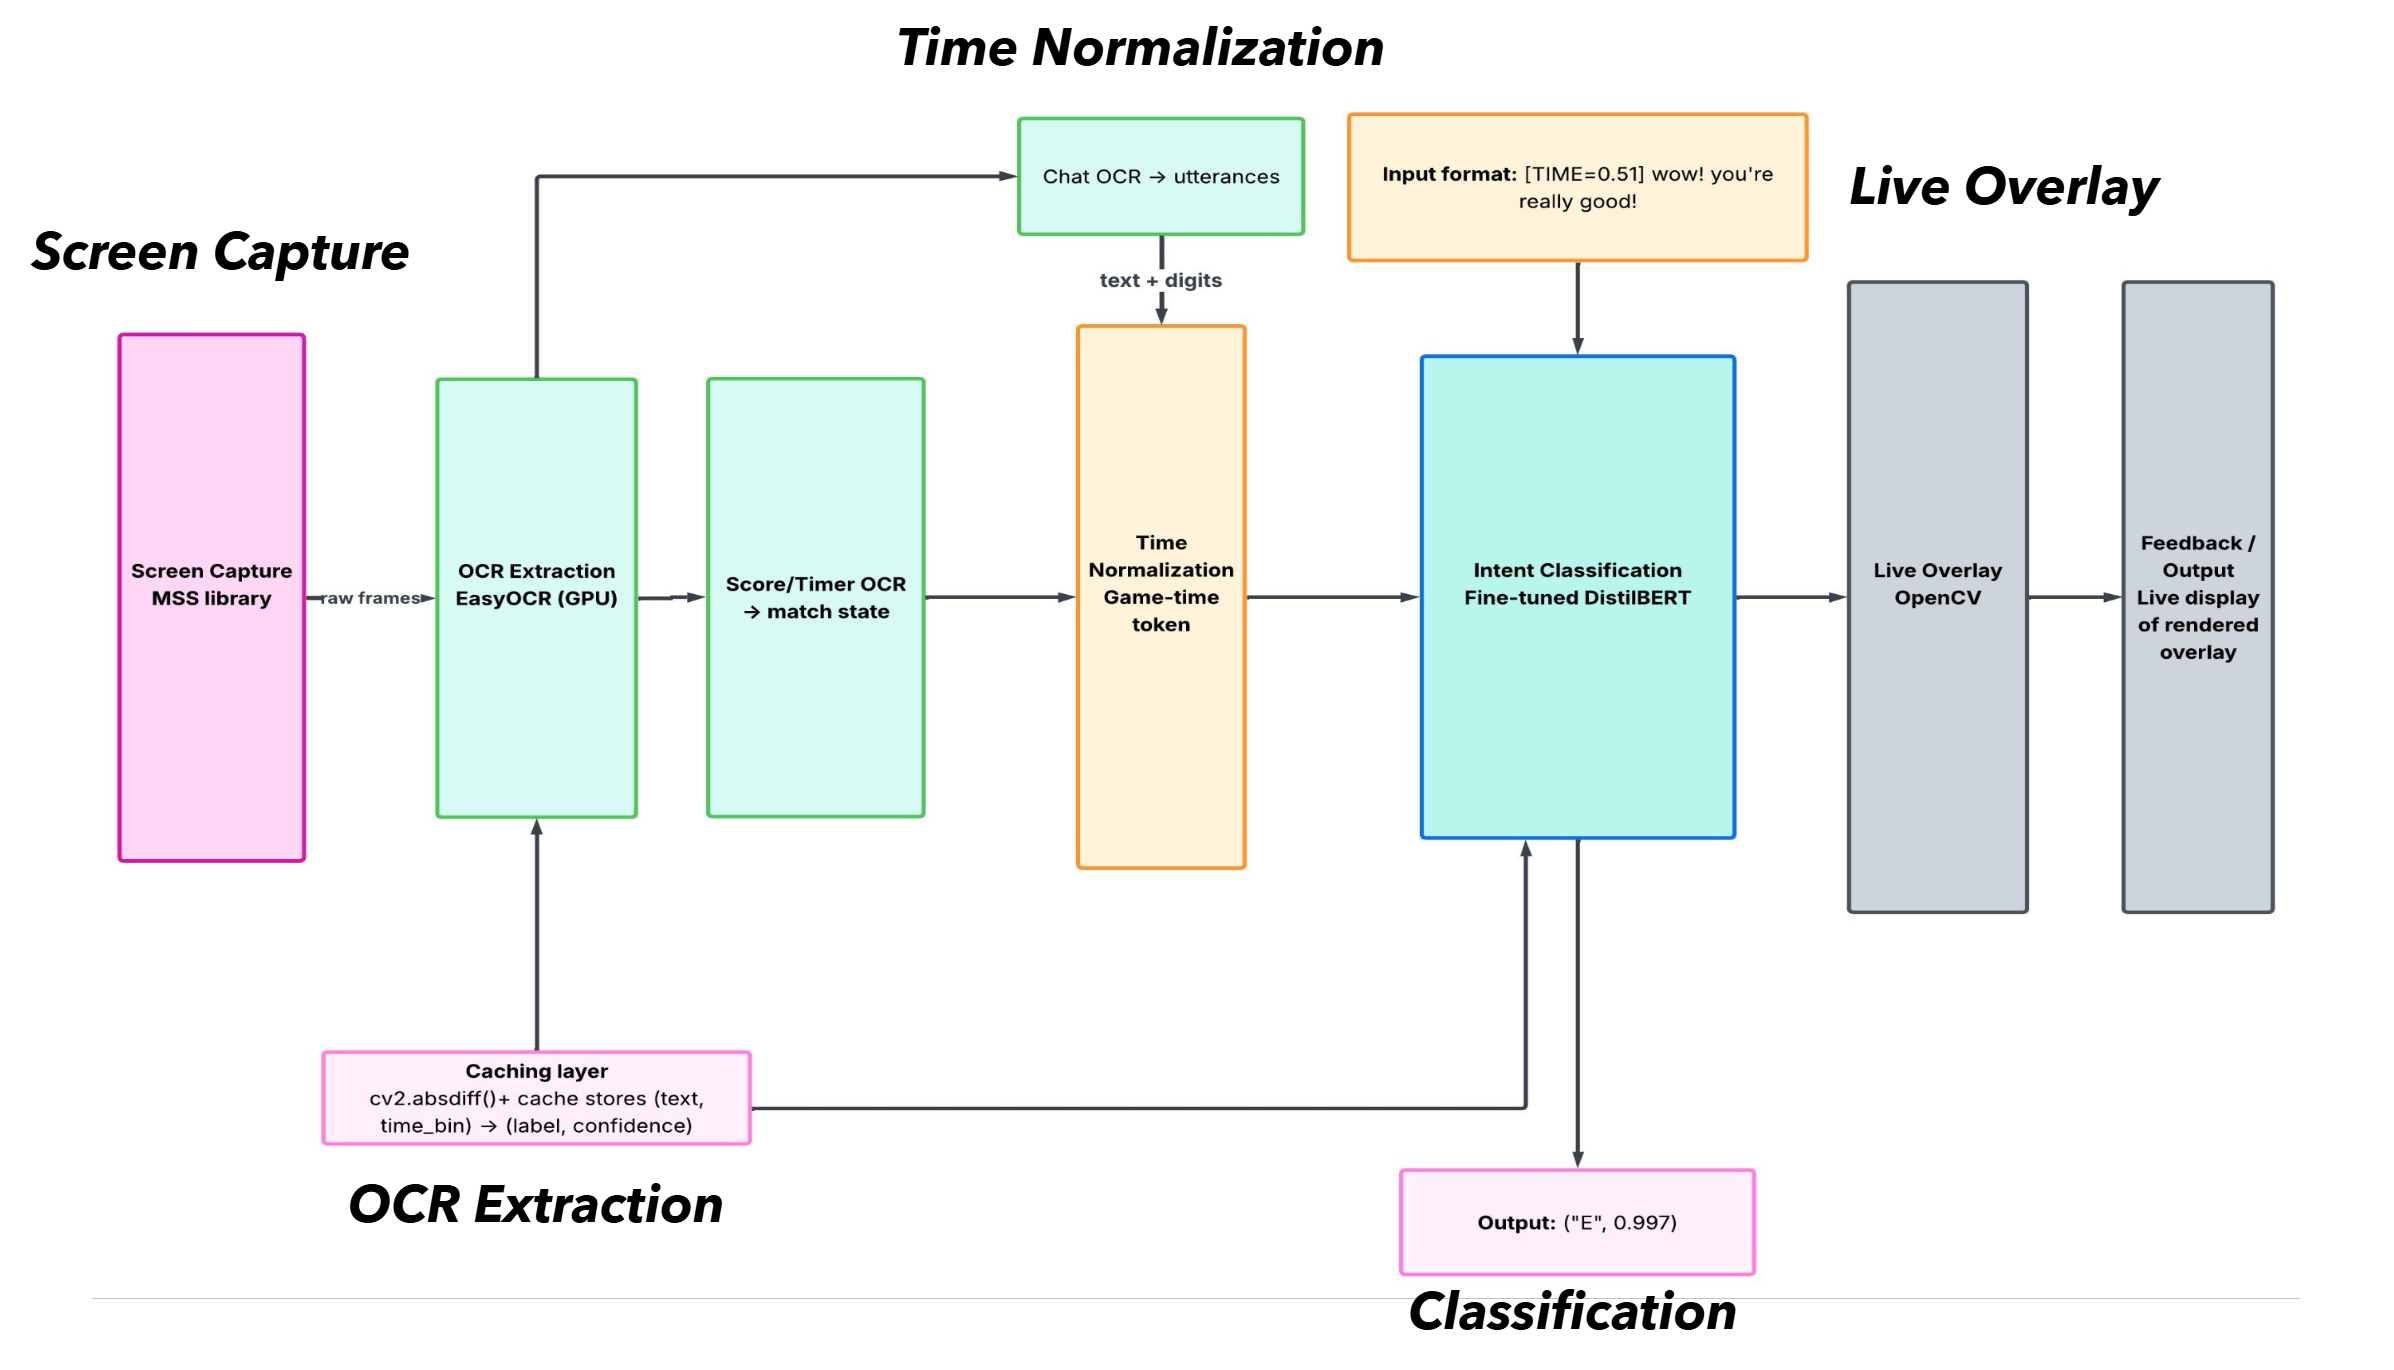
\includegraphics[width=1\linewidth]{Pipeline.png}
    \caption{Live deployment pipeline: per-frame stages from screen capture through transparent overlay.}\label{fig:pipeline}
\end{figure}


\section{Experimental setup}

\subsection{Training hyperparameters}

\begin{table}[H]
    \centering
    \begin{tabular}{@{}l l@{}}
    \toprule
    \textbf{Hyperparameter} & \textbf{Value} \\
    \midrule
    Optimizer           & AdamW \\
    Learning rate       & $2 \times 10^{-5}$ \\
    Batch size          & 32 \\
    Max sequence length & 64 tokens \\
    Epochs              & 5 \\
    Gradient clipping   & max-norm 1.0 \\
    Loss                & Class-weighted cross-entropy \\
    Random seed         & 42 \\
    \bottomrule
    \end{tabular}
    \caption{Training hyperparameters for the DistilBERT-CONDA fine-tune.}\label{tab:hparams}
\end{table}

\subsection{Hardware and software}

Training and evaluation were run on a single CUDA-enabled GPU using PyTorch and HuggingFace Transformers. The live pipeline also runs on the same hardware, with EasyOCR also using the GPU when available.

\subsection{Metrics}

We report the two metrics used by the original CONDA paper:
\begin{itemize}
    \item \textbf{UCA}: utterance-level classification accuracy (overall accuracy across all four classes).
    \item \textbf{Per-class U-F1}: one-vs-rest F1 for each of E, I, A, O.
\end{itemize}

Additionally I report \textbf{macro-F1} (unweighted mean of per-class F1), because of the class imbalance UCA is dominated by the 74\% O class and overstates performance.

\subsection{Conditions}

I compared two model variants, identical except the input format:
\begin{itemize}
    \item \textbf{No-time:} raw utterance fed to DistilBERT.
    \item \textbf{With-time:} \texttt{[TIME=x.xx]} prefix prepended to the utterance.
\end{itemize}

Both variants are trained for 5 epochs with seed 42, and the best checkpoint by validation macro-F1 is what is selected.

\section{Results}

\subsection{Headline numbers}

Validation results for the two conditions are shown along with the JointBERT baseline from Weld et al. (2021) in Table~\ref{tab:headline}. Note that those numbers are from the held-out test set whose labels are not publicly available, so the comparison is not strictly apples-to-apples.

\begin{table}[H]
    \centering
    \small
    \begin{tabular}{@{}l r r r r r r@{}}
    \toprule
    \textbf{Model} & \textbf{UCA} & \textbf{Macro-F1} & \textbf{F1[E]} & \textbf{F1[I]} & \textbf{F1[A]} & \textbf{F1[O]} \\
    \midrule
    JointBERT (Weld 2021)\textsuperscript{*}        & 0.921           & n/a             & 0.872           & 0.768           & 0.800           & 0.954           \\
    \textbf{DistilBERT, no time}                    & \textbf{0.9133} & \textbf{0.8375} & \textbf{0.8590} & \textbf{0.7426} & \textbf{0.7994} & \textbf{0.9490} \\
    DistilBERT, with \texttt{[TIME]}                & 0.9112          & 0.8331          & 0.8573          & 0.7388          & 0.7884          & 0.9480          \\
    \bottomrule
    \end{tabular}
    \caption{Validation results on CONDA. JointBERT numbers are from the CONDA paper (test set).}\label{tab:headline}
\end{table}

\noindent\textsuperscript{*}JointBERT numbers are reported on the held-out CONDA test set; ours on the validation set.

\begin{figure}[H]
    \centering
    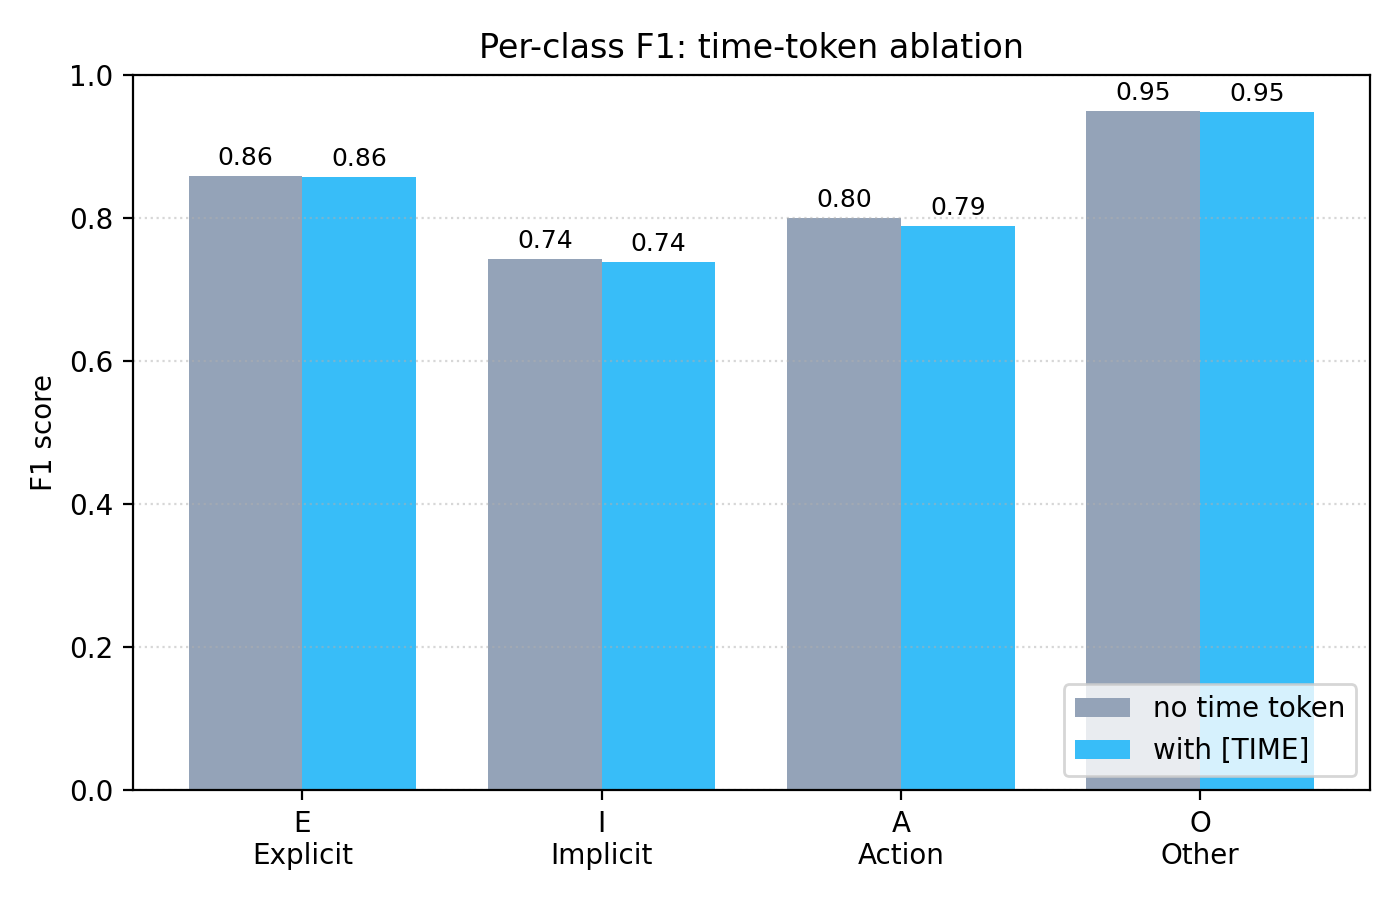
\includegraphics[width=0.8\linewidth]{per_class_f1.png}
    \caption{Per-class F1 on the CONDA validation set: no-time vs with-time DistilBERT.}\label{fig:per_class_f1}
\end{figure}

Three observations:
\begin{enumerate}
    \item \textbf{The single-task DistilBERT model is competitive with the dual-task JointBERT baseline.} UCA is within 0.8 points; F1[A] is essentially tied (0.7994 vs 0.800); F1[O] is within 0.5 points; F1[E] is within 1.3 points. The largest gap is on F1[I] (2.5 points), the hardest class for both models. Achieving this without slot-level supervision is, in my view, the most practically meaningful result of the project.
    \item \textbf{The game-time token does not help.} Every metric is worse with the \texttt{[TIME]} prefix than without: UCA $-$0.21 pts, macro-F1 $-$0.44 pts, and per-class F1 deltas of $-$0.17 (E), $-$0.38 (I), $-$1.10 (A), $-$0.10 (O). The differences are small but consistent and in the same direction across all four classes.
    \item \textbf{The largest changes are on the rarer classes (A and I).} This is consistent with my thoughts early on that the rare classes have the least redundancy in their lexical signal and are the most sensitive to noise introduced by the time prefix.
\end{enumerate}

\subsection{Per-class confusion analysis}

The confusion matrix for the with-time model (label order E / I / A / O) is shown in Table~\ref{tab:confusion}.

\begin{table}[H]
    \centering
    \begin{tabular}{@{}l r r r r r@{}}
    \toprule
                  & \textbf{pred E} & \textbf{pred I} & \textbf{pred A} & \textbf{pred O} & \textbf{total} \\
    \midrule
    true E        & 1045 &  24 &  27 &   87 & 1183 \\
    true I        &   23 & 427 &  16 &  116 &  582 \\
    true A        &   18 &   7 & 488 &   67 &  580 \\
    true O        &  169 & 116 & 127 & 6216 & 6628 \\
    \bottomrule
    \end{tabular}
    \caption{Confusion matrix on validation, with-time model. Rows are true labels, columns are predictions.}\label{tab:confusion}
\end{table}

\begin{figure}[H]
    \centering
    \begin{minipage}{0.48\linewidth}
        \centering
        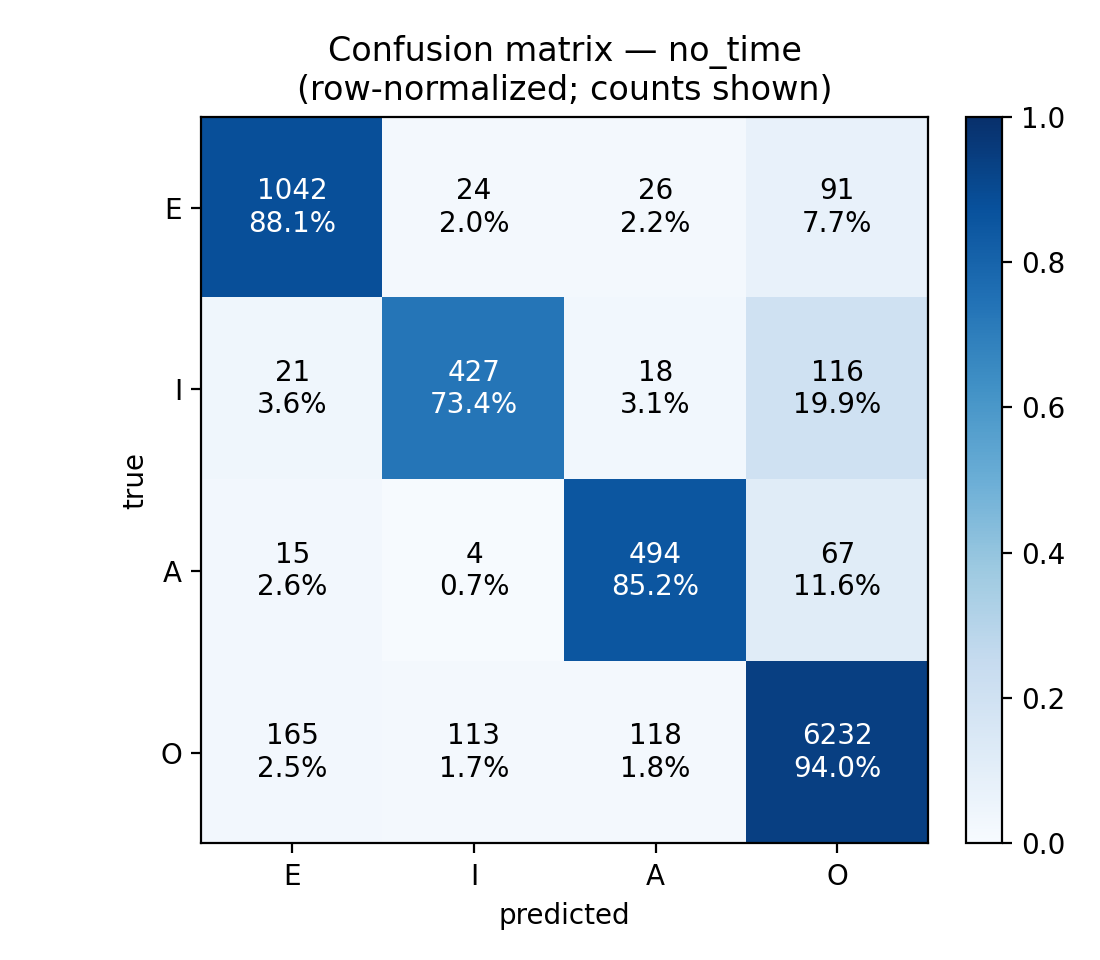
\includegraphics[width=\linewidth]{confusion_no_time.png}
        \subcaption{No-time model}\label{fig:cm_no_time}
    \end{minipage}\hfill
    \begin{minipage}{0.48\linewidth}
        \centering
        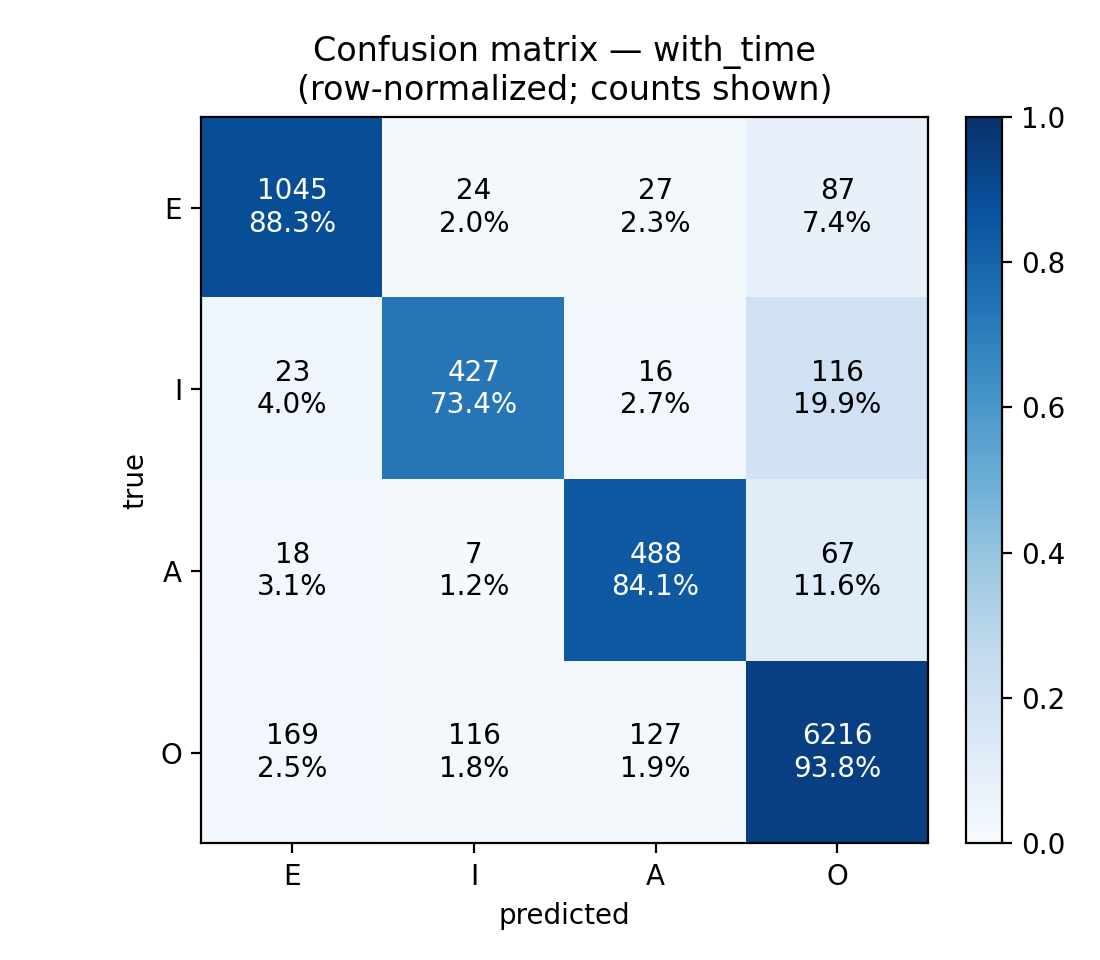
\includegraphics[width=\linewidth]{confusion_with_time.png}
        \subcaption{With-time model}\label{fig:cm_with_time}
    \end{minipage}
    \caption{Row-normalized confusion matrices on the CONDA validation set; counts and row percentages are shown in each cell.}\label{fig:confusion}
\end{figure}

Two failure modes dominate:
\begin{itemize}
    \item \textbf{I to O leakage (116 / 582 = 20\%).} Implicit toxicity by definition lacks the explicit language and obscenities that flag E utterances; its grammatical construction is often hard to distinguish from neutral chat. Examples like ``not a good pudg'' or ``wtf are you doing'' are flagged by humans because of context, not vocabulary. This is the failure mode the CONDA authors identified, and the one we hoped a temporal prior might help with. The time token, in the event, did not.
    \item \textbf{A to O leakage (67 / 580 = 12\%).} Action calls such as (``pause, line crossed'', ``gg reporting'') I feel overlap with neutral coordination talk and because of this get absorbed into the dominant \emph{Other} class.
\end{itemize}

E is the cleanest category, with only \textasciitilde{}12\% of true E utterances being misclassified. Explicit toxicity has a more distinguishable structure that the model picks up reliably.

\subsection{Training dynamics}

Training curves for both runs (Figure~\ref{fig:training_curves}) show a familiar pattern:
\begin{itemize}
    \item Training loss declines smoothly from \textasciitilde{}0.75 at epoch 1 to \textasciitilde{}0.19 at epoch 5.
    \item Validation loss declines through epoch 2 then rises (\textasciitilde{}0.47 $\rightarrow$ \textasciitilde{}0.65) as the model begins to overfit.
    \item Validation macro-F1 continues to improve through epoch 5 despite the rising validation loss.
\end{itemize}

\begin{figure}[H]
    \centering
    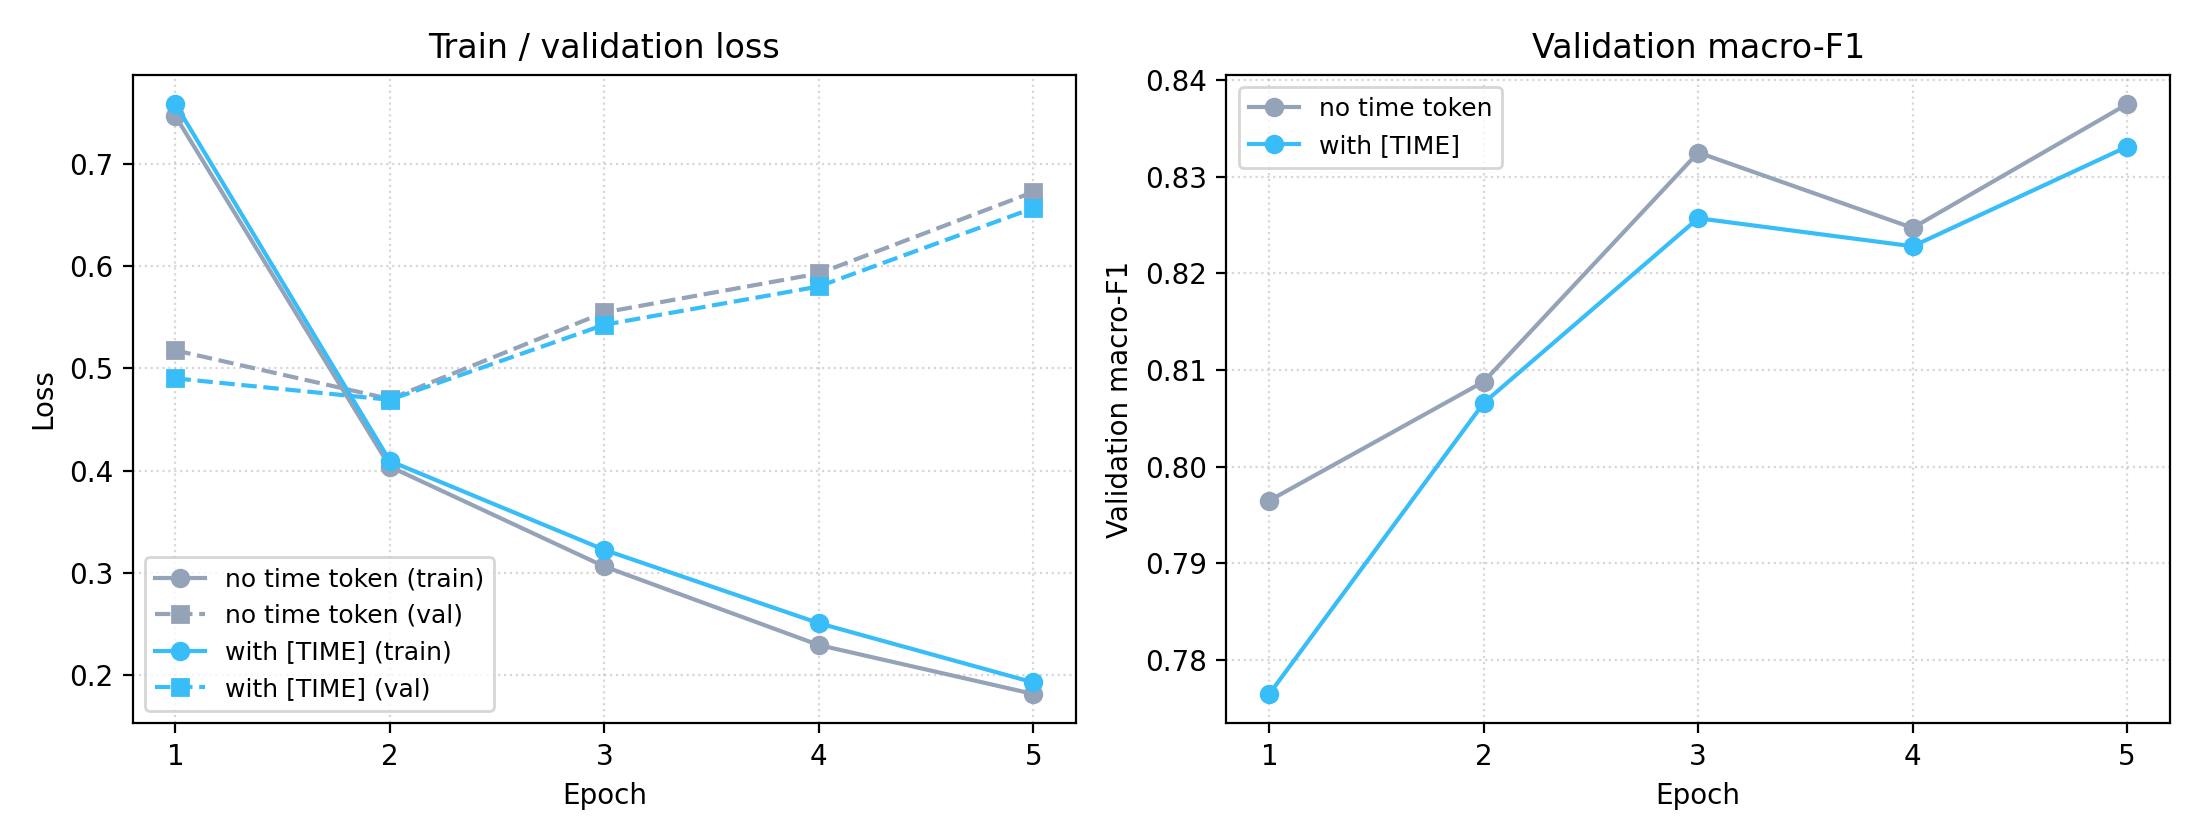
\includegraphics[width=\linewidth]{training_curves.png}
    \caption{Training and validation loss (left) and validation macro-F1 (right) across 5 epochs for both runs.}\label{fig:training_curves}
\end{figure}

This rising loss alongside improving F1 is most likely due to the model becoming over-confident on examples it gets right (raising loss) while still flipping rare-class examples from wrong to right (raising F1). Because I selected macro-F1 rather than loss, this is the correct behaviour, but it shows we are training right at the edge: a slightly longer schedule would likely start deteriorating F1 too.

\section{Discussion}\label{sec:discussion}

\subsection{Why the game-time token failed}\label{sec:why-time-failed}

In the beginning our hypothesis was that, because the live pipeline classifies utterances one at a time and loses the conversational context that JointBERT-style models can exploit, a normalised game time additive could serve as a way of making up for this contextual loss for ``where in the match are we'' and shift the prior over intent classes accordingly (M\"artens et al.\ 2015 having shown that toxicity is non-uniform in time). This hypothesis was not supported. Several factors can explain the negative result:

\paragraph{Tokenisation waste.} The \texttt{[TIME=0.84]} prefix consumes roughly seven of the 64 available tokens. For utterances near the limit, this is a critical part of the model's input budget not involved with the actual content.

\paragraph{Subword fragmentation.} Because we did not register \texttt{[TIME]} as a single special token, the prefix is shattered by WordPiece into \texttt{[}, \texttt{time}, \texttt{=}, \texttt{0}, \texttt{.}, \texttt{8}, \texttt{4}, \texttt{]}. The model has to learn temporal signal across many positions and many digit-subword embeddings, none of which were pre-trained on numeric scalars. A registered special token, ideally with an embedding initialised on a temporal, would be a cleaner test for our model.

\paragraph{Redundancy with lexical signal.} Our no-time model is already at macro-F1 $\sim$0.84. The cues for the four classes are strong: explicit language are heavily gauged towards E; ``gg'' and ``uninstall'' near the end of a match are easy lexical patterns; coordination calls like ``smoke'', and ``rotate'' are A. There is little signal margin left for a temporal feature to add.

\paragraph{Match-time scalar may not encode the right thing.} M\"artens et al.\ (2015) found that toxicity spikes are event-triggered such as post-death and post-team-fight rather than only related to elapsed time. A normalised value in $[0, 1]$ cannot capture an event-triggered spike unless events happen at predictable times, which they do not. An expansion of this project would be taking into account these events.

\paragraph{CONDA's labels are content-conditional, not time-conditional.} Looking at the dataset shows that label assignment depends almost entirely on the surface content of the utterance. This means that match time is not weighed when this data was labelled. Of 258 utterance texts repeated five or more times in the training split, 232 (89.9\%) carry one label on at least 90\% of occurrences. The utterances we would most expect to vary in meaning with match time do not vary in their labels: ``gg'' is labelled O on 1376 of 1378 occurrences, ``gg wp'' on 277 of 277, ``?'' on 343 of 343, and ``:D'' on 120 of 120. Making \texttt{chatTime} into six equal-width intervals and computing the conditional label distribution per bin, $P(O \mid \text{bin})$ stays within $[0.727, 0.760]$ against a marginal of $0.742$, and the mean Kullback--Leibler divergence from the marginal across bins is $0.006$ bits. A chi-squared test of independence rejects the null at $p = 1.2 \times 10^{-38}$, but this is driven by sample size ($N = 26{,}914$) rather than practical effect size. The implication is that the temporal signal a time token would need to exploit is not encoded in the labels: even a perfectly designed temporal feature cannot help the model recover information the annotators did not condition on. This is plausibly the dominant reason for our negative result, and unlike the four mechanisms above it is specific to CONDA rather than a generic argument about temporal conditioning. The natural follow-up is to re-annotate a subset of CONDA with explicit instruction to consider match-time context, then re-run the time-token ablation against the re-annotated labels.

We therefore frame the time-token result as: a subword-fragmented match-time scalar does not improve utterance-level intent classification on CONDA, and we identify five reasons that likely contributes to that result, the most important of which is that CONDA's labels are themselves content-bound rather than time and content bound. The broader hypothesis, that some form of temporal or event-based conditioning could help, is not refuted by this experiment; testing it properly would require a dataset whose labels pay attention to temporal context.

\subsection{Single-task vs.\ dual-task supervision}

The competitive performance of our single-task model relative to JointBERT is worth looking at. JointBERT receives both intent labels and token-level slot labels during training, and is generally expected to benefit from these. My intent-only model lands within 0.8 UCA points of it suggesting that, either (a) DistilBERT's representations are strong enough to recover most of the discriminative signal that slot labels provide, or (b) the marginal benefit of slot supervision on CONDA is smaller than the JointBERT vs vanilla-BERT comparison in the original paper might suggest. For a deployment pipeline where slot-level annotations are unavailable at inference time anyway, this is a useful finding: the simpler architecture is good.


\section{Limitations}\label{sec:limitations}

We are upfront about the following limitations of the current work:

\begin{itemize}
    \item \textbf{Single seed.} All reported numbers are from a single training run with seed 42. Multi-seed evaluation is required before any claims about model performance can be made with confidence. It's noted that for the time-token result specifically, the seed-variance concern is at least partly subordinate to the dataset-structure concern in the next bullet: a result that the labels cannot encode is unlikely to change direction across seeds.

    \item \textbf{The time-token ablation is bounded by CONDA's annotation structure.} As detailed in \S\ref{sec:why-time-failed}, CONDA's labels are essentially invariant to match time. Our experiment therefore cannot distinguish between (a) match-time conditioning being unhelpful in principle and (b) match-time conditioning being unhelpful for \emph{this} labelset. A re-annotation experiment with explicit time-context instructions to annotators would be needed to resolve the ambiguity; we discuss this further in \S\ref{sec:future-work}.

    \item \textbf{Validation-set evaluation only.} CONDA's test labels are withheld; we evaluate on validation throughout. This means our headline numbers are not directly comparable to the test-set numbers reported by the original CONDA authors, and we may be slightly optimistic where validation/test distribution differences favour validation.

    \item \textbf{Cross-domain transfer is untested.} The model is trained on Dota 2 chat (CONDA) and deployed live on VALORANT. Slang overlap is partial: \texttt{gg}, \texttt{ez}, \texttt{noob} transfer; hero/agent names, item names, and game-specific callouts do not. A held-out VALORANT chat evaluation set is the proper way to characterise this gap, and we have not built one.

    \item \textbf{OCR error propagation is unquantified.} Real-world OCR introduces character substitutions, deletions, and segmentation errors. We have not measured the relationship between OCR character error rate and downstream classification accuracy. An OCR-noise robustness study (training-time augmentation and/or test-time perturbation) was scoped out for time.

    \item \textbf{VALORANT-specific time arithmetic.} The match-time reconstruction (\texttt{completed\_rounds $\times$ 100 + (100 $-$ round\_seconds)}) assumes 100-second VALORANT rounds and a (won, lost) scoreboard. It is not portable to Dota 2 (continuous match clock) or other titles without a per-game rewrite.

    \item \textbf{Pixel-coordinate-bound ROIs.} ROIs are hand-coded for one screen resolution and one game UI. A different resolution, windowed mode, or UI-scale setting breaks the OCR step.

    \item \textbf{Pause and intermission states.} Bomb-plant freezes, half-time, and overtime transitions are handled with a coarse 15-second sleep heuristic rather than detected explicitly.

    \item \textbf{Auto-blocked words.} The game client filters certain slurs and obscenities before they reach the chat UI; the model never sees these in deployment, only in training. We have not characterised the resulting train/deploy distribution shift.

    \item \textbf{No cased-vs-uncased ablation.} We chose \texttt{distilbert-base-cased} on a priori grounds (uppercased gameplay tokens carry signal) but did not run the controlled experiment.
\end{itemize}


\section{Future Work}\label{sec:future-work}

Four extensions would meaningfully strengthen the project:

\begin{enumerate}
    \item \textbf{Re-annotation of a CONDA subset with time-context instructions.} This is the most important next step and follows directly from the finding in \S\ref{sec:why-time-failed}. A subset of CONDA (e.g., 2000 utterances stratified across \texttt{chatTime} bins) would be re-annotated with explicit guidance that annotators may, and should, consider match-time context when assigning intent. The hypothesis is that early-match ``gg'' should land in E or I more often than late-match ``gg'', and that re-annotation will surface a time-conditional component to the label distribution that the original guidelines suppressed. The time-token ablation would then be re-run against the re-annotated labels, providing a genuine test of whether temporal conditioning helps when the labels themselves carry temporal information.

    \item \textbf{Multi-seed evaluation.} Three seeds (e.g., 42, 7, 123) would let us report mean $\pm$ std and a paired test on per-example correctness, putting all quantitative results on statistical footing. This is independently valuable regardless of which dataset the time-token ablation is re-run on.

    \item \textbf{A better-designed temporal-conditioning experiment.} Register \texttt{[TIME]} as a single special token with a dedicated embedding, addressing the subword-fragmentation mechanism identified in \S\ref{sec:why-time-failed}. Consider also conditioning on event-proximity features (time-since-last-death, time-since-last-team-fight), which are theoretically better aligned with M\"artens et al.'s findings than a global match-time scalar. This experiment is most informative when paired with re-annotated labels (item 1); on the original CONDA labels it would likely reproduce the negative result reported here.

    \item \textbf{OCR-robustness characterisation.} Train and evaluate on synthetically perturbed text (random character swap/delete at 5\%, 10\%, 20\%) to characterise end-to-end robustness. This is the contribution most directly relevant to deployment and is a small project in itself.
\end{enumerate}

Beyond these, a Dota-2-deployment evaluation (closing the train/deploy domain match) and a quantified end-to-end latency budget would round out the experimental story.


\section{Conclusion}\label{sec:conclusion}

We built and evaluated an end-to-end pipeline for real-time intent classification of in-game chat. A single-task DistilBERT model fine-tuned on CONDA achieves macro-F1 0.8375 / UCA 0.9133 on the validation set, competitive with the dual-task JointBERT baseline despite using only intent-level supervision. A controlled ablation of normalised game-time conditioning, prepending \texttt{[TIME=x.xx]} to each utterance, produced a small but consistent negative effect across all four classes (UCA $-$0.21 points, macro-F1 $-$0.44 points, per-class F1 between $-$0.10 and $-$1.10 points). While engineering factors like subword fragmentation of the time prefix and redundancy with already-strong lexical signal likely contribute to this result, dataset analysis points to a more fundamental cause: CONDA's labels are essentially invariant to match time, with 89.9\% of repeated utterances carrying a single dominant label regardless of when in the match they appear. The temporal signal a time token would need to exploit is therefore not present in the labels, and no engineering refinement of the time feature can recover information the annotators did not condition on.

The system runs end-to-end on a live VALORANT window, with an overlay surfacing per-utterance classifications. The system's limitations are documented openly that the single-seed evaluation, untested cross-domain transfer, and unquantified OCR robustness, and identified the experiments that would address each, with re-annotation of CONDA under time-aware context as the most important next step.

% BIBLIOGRAPHY: Create or upload a bib file to manage your references. For instructions, see www.overleaf.com/learn/how-to/Using_bibliographies_on_Overleaf. Citations will use the Chicago Manual of Style notes and bibliography citation format, described at www.chicagomanualofstyle.org/tools_citationguide/citation-guide-1.html.

\nocite{*}
\printbibliography[title={References}]

\end{document}
